% %!TEX root=../template.tex

\begin{figure}[t]
\centering
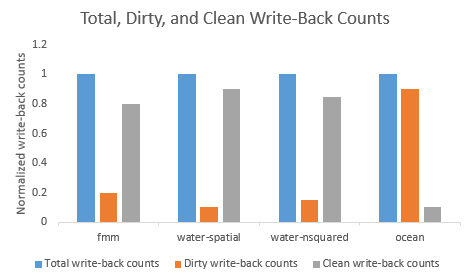
\includegraphics[width=\columnwidth]{figs/cleancount}    
%\includegraphics[trim=0 0 0 0, clip, width=\columnwidth]{figs/browser-arch}
\caption{Dirty and Clean Write-Back Analysis}
\label{fig:cleancount}
\end{figure}


\begin{figure}[t]
\centering
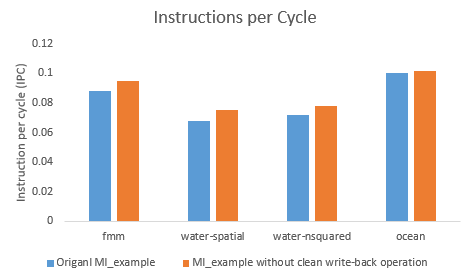
\includegraphics[width=\columnwidth]{figs/ipc}    
%\includegraphics[trim=0 0 0 0, clip, scale=0.5, width=\columnwidth]{figs/browser-arch}
\caption{Performance Result}
\label{fig:ipc}
\end{figure}



\subsection{Clean Write back Avoidance}
~\Fig{fig:cleancount} shows the results of dirty write back counts and clean write back counts based on splash 2 benchmark, which is tested with ruby option enabled in gem5 using MI\_example 1 level cache coherence. We can see there is large number of clean write back, almost 90\% in fmm, water-spatial and water-nsquared benchmark, which means these cache blocks are no modified so still written back to higher memory hierarchy, so reducing these unnecessary write will help to increase system performance and reduce power. But we should note that different benchmarks have different characteristics, so the percentage of clean write back is different.  

After modify the coherence protocol in MI\_example file of gem5 to remove unnecessary clean write back, we calculate number of cycle and number of instruction running by the benchmark. We can see in ~\Fig{fig:ipc} that IPC of each benchmark has different level of improvement, which is proportional to the percentage of clean write back in the benchmark. For example, the benchmark:"ocean" has a little clean write-back operation, so it doesn't have obvious performance improvement. 
Coherence protocol is very important in today's multicore 



\begin{figure}[t]
\centering
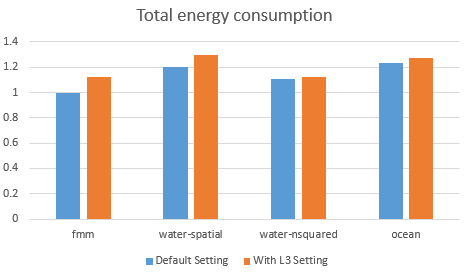
\includegraphics[width=\columnwidth]{figs/l3power} 
%\includegraphics[trim=0 0 0 0, clip, scale=0.5, width=\columnwidth]{figs/browser-arch}
\caption{Power Consumption Compare with L3}
\label{fig:l3power}
\end{figure}


\subsection{L3 Cache}

L3 cache is important in modern computer system, we integrate L3 cache into gem5 to see its impact on performance and power. We compare the gem5 default architecture and the architecture with L3 cache, in ~\Fig{fig:l3power} we can see there some increase of power for L3 cache in the benchmark, because additional L3 cache will incur more dynamic and static power. The power is normalized based on default gem5 architecture as baseline. But this architecture can be used in our following experiment as fundamental gem5 setting. Also, we also see different benchmarks have different impact on the performance and power based on their different property.       



\begin{figure}[t]
\centering
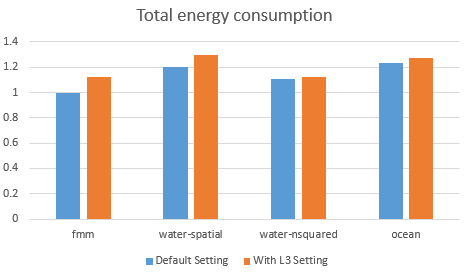
\includegraphics[width=\columnwidth]{figs/l3power} 
%\includegraphics[trim=0 0 0 0, clip, scale=0.5, width=\columnwidth]{figs/browser-arch}
\caption{ Cache Replacement Policy Power Compare}
\label{fig:replace}
\end{figure}



\subsection{Cache Replacement Policy}
In this experiment, we replace LRU replacement policy in cache with different replacement policy, especially NMRU, LIP and Random replacement policy. In ~\Fig{fig:replace} we can see that the default LRU is still perform well and has better power benefit and random replacement policy. The benefit of LIP and NMRU is varying based on the property of benchmark. For example, if the benchmark size is larger than cache size, LIP will have more benefit than LRU because it will select the least recently used block as replacement. The power is normalized using LRU as baseline. 



\begin{figure}[t]
\centering
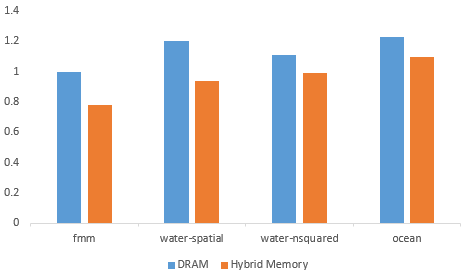
\includegraphics[width=\columnwidth]{figs/hybridpower} 
%\includegraphics[trim=0 0 0 0, clip, scale=0.5, width=\columnwidth]{figs/browser-arch}
\caption{Power Compared with DRAM and Hybrid Memory}
\label{fig:hybridpower}
\end{figure}


\subsection{Hybrid Memory}
In order to analyze the power and performance behavior of hybrid NVM, the power is normalized using traditional DRAM as baseline. Regarding the leakage power, there is a significant gain is observed replacing three channel DRAM with three channel NVM and one channel DRAM. Thus, we can see there is energy saving in the benchmark as shown in ~\Fig{fig:hybridpower}. The NVMain simulator setting corresponding NVM configuration and DRAM configuration. Due to time limit, we expect to change to ratio of NVM in hybrid memory to observe some change. But there is also some overhead for memory controller to schedule data to different kind of memory. Also, if data if constantly write into NVM, it will incur additional power consumption, which may offset the power saving from leakage reduction. Thus, an efficient memory controller is important especially in hybrid memory  system. 















